\chapter{Design of Web Elements}\label{cha:web}

\section{Web Workers}

    

\section{Message Stacks}

    Circular Stack \ac{LIFO}

    \begin{figure}[htbp]
        \centering
        \begin{subfigure}[t]{0.32\textwidth}
            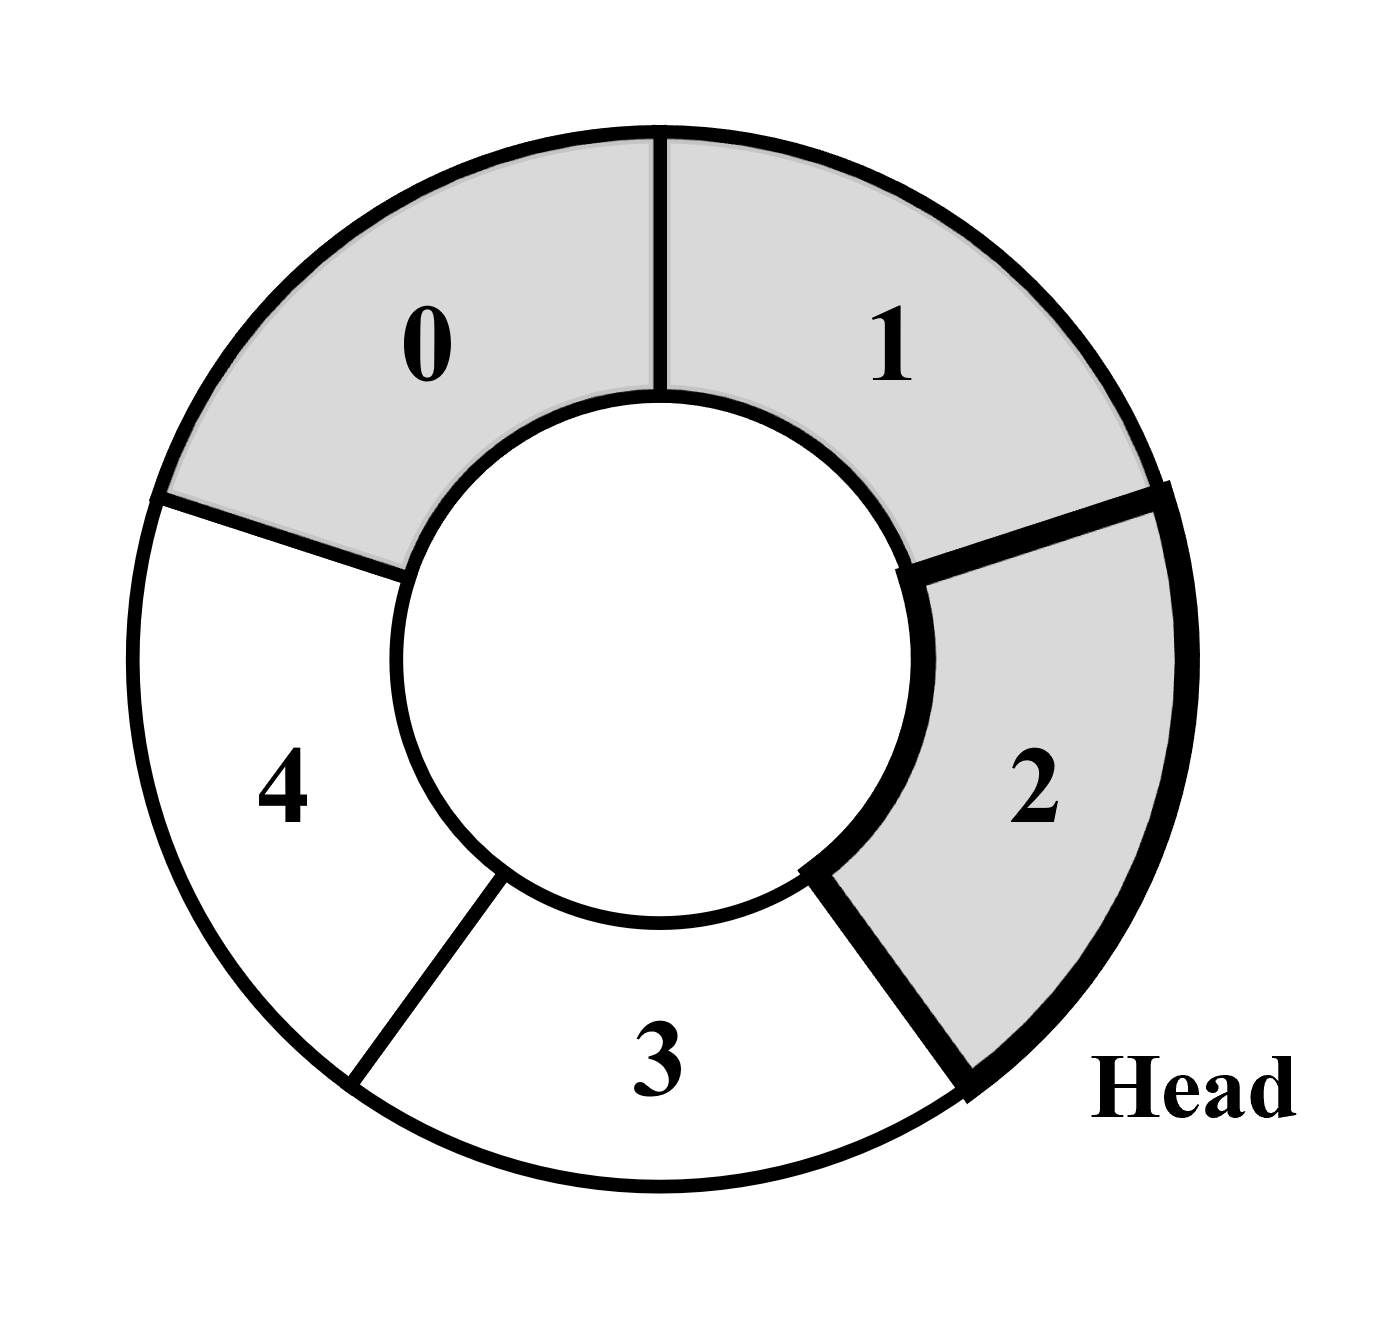
\includegraphics[height=0.9\textwidth]{07_stack0.png}
            \caption{Filling stack}
        \end{subfigure}
        \begin{subfigure}[t]{0.32\textwidth}
            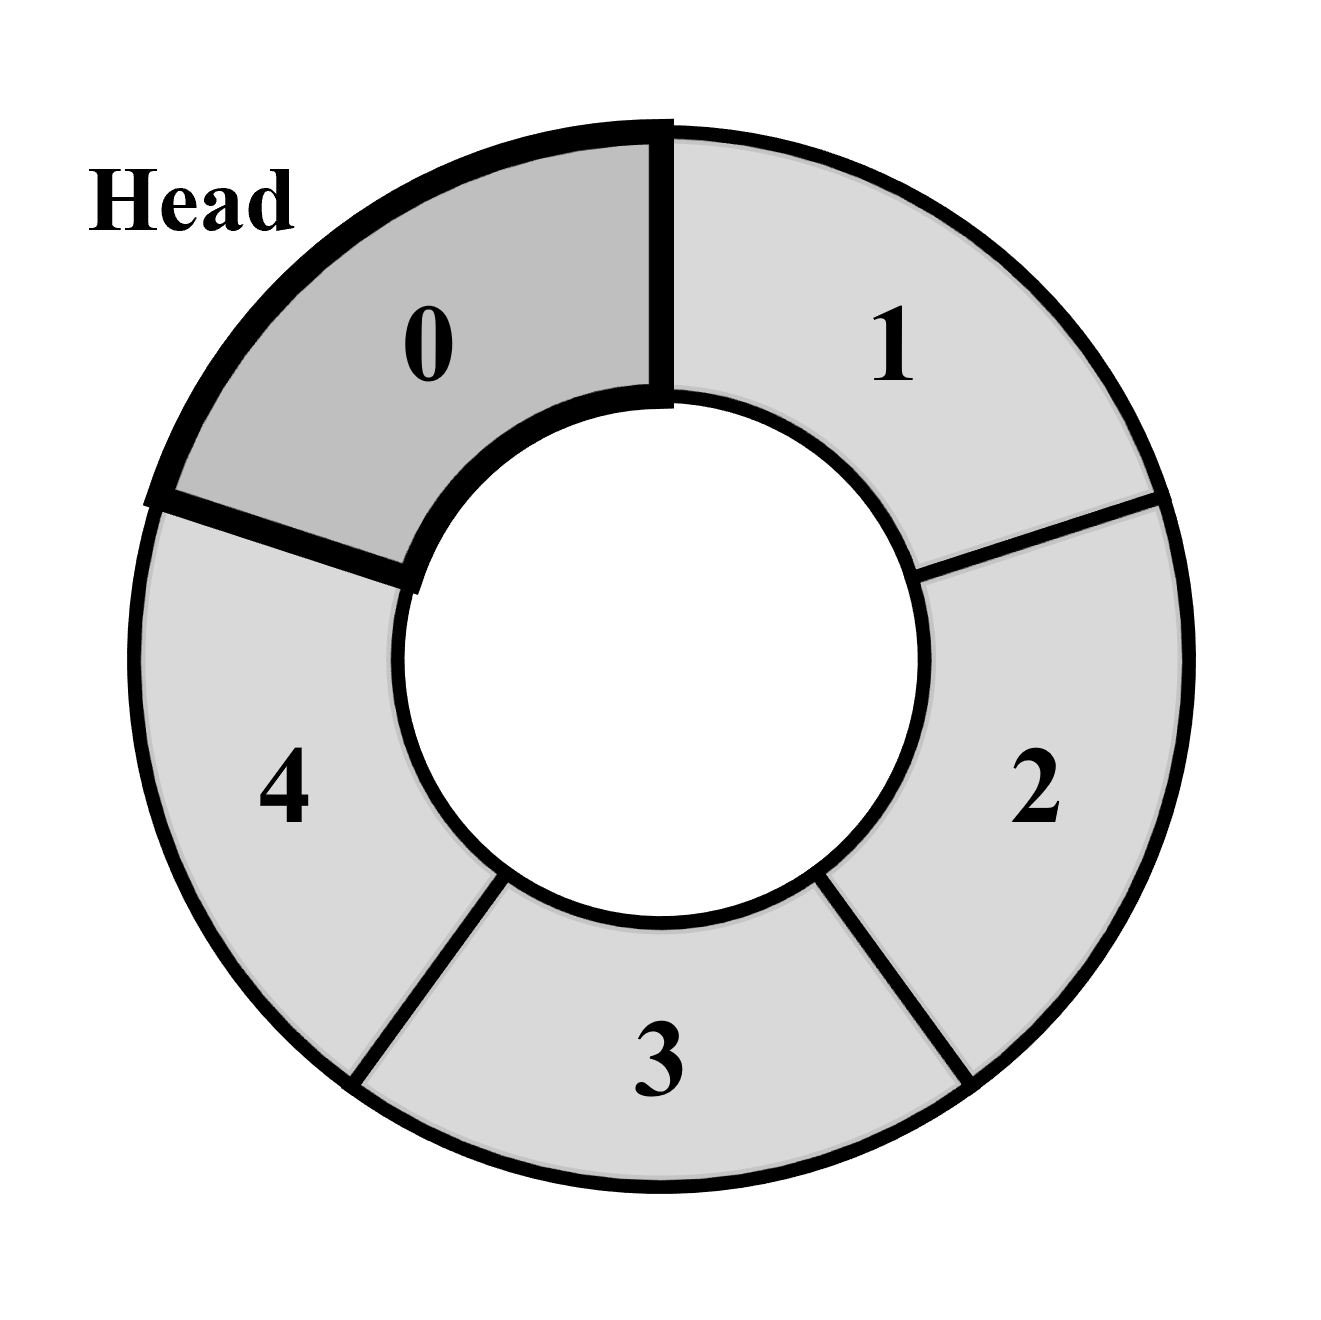
\includegraphics[height=0.9\textwidth]{07_stack1.png}
            \caption{Overwriting stack}
        \end{subfigure}
        \begin{subfigure}[t]{0.32\textwidth}
            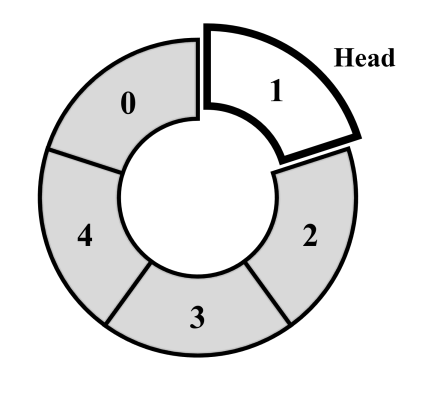
\includegraphics[height=0.9\textwidth]{07_stack2.png}
            \caption{Reading stack}
        \end{subfigure}
        \caption{TODO:}\label{fig:circleStack}
    \end{figure}

- Web workers, what are they? why are they needed?
- Communication channels
- Registry of topics/subs/pubs
- Message handling
width